\subsection{Clustering}
\label{sec:clustering}

In machine learning, decision trees are classified as a supervised learning method, and the first step towards designing them requires that the data be labeled according to their attributes. The inherent attribute of our data are the GOF value themselves, but because of the multiplicity of metrics and lack of clarity about how these relate to each other, we need to add labels to the data that are in accordance with our predefined validation categories. We label the data in our dataset by means of a clustering process. 

In general, clustering is an unsupervised approach used to group data points in a multi-dimensional space, based on the similarity of their attributes. Clustering is considered an exploratory activity as a part of a data mining process \citep{Fayyad_1996_IEEE}. It yields clusters of data with distinctive attribute patterns. \citet{Jain_1999_ACMCS} classifies clustering approaches into two categories: hierarchical and partitional. Aside from other technical details, the basic difference between them is that hierarchical algorithms create nested partitions whereas partitional algorithms produce singular partitions. 

Admittedly, there is not a single clustering assignment that can explain every dataset, which makes clustering an application dependent process \citep{Dy_2004_MLR, Jain_1988_Book, Hartigan_1985_JOC}. Consequently, one needs to make choices. We use a partitional, distance-based method known as constrained \kmeans{}. The standard \kmeans{} method is a process for partitioning a $n$-dimensional population into $k$ clusters with a minimum within-cluster attributes variance \citet[e.g.,][]{Macqueen_1967_Proc}. 

Given a $k$ number of clusters, where each cluster is identified by its center location, the process starts by computing the distances of all other data-points to the center of the clusters and grouping them based on the proximity to the clusters' centers. Once this is done, the center of the cluster is updated based on the attributes of the data-points in each cluster. The process is then repeated iteratively until the data-points in each cluster becomes stable in regards to the variation of the center's location with respect to the previous iteration (down to a given tolerance). 

The standard \kmeans{} process is, however, sensitive to the initial selection of the clusters and their centers' location. To partially mitigate this, the constrained \kmeans{} method introduces two types of constraints: must-link and cannot-link \citep{Wagstaff_2001_Proc}. The must-link constraint specifies instances in which data must be linked to a specific cluster. The cannot-link constraint, on the other hand, specifies instances in which data cannot be within the same cluster. This prevents the clustering process from converging into a local minimum. Figure \ref{fig:k-means} illustrates the differences between the standard and constrained \kmeans{} methods for a single clustering iteration on a small dataset.

The clustering process can be further refined, based on background information about the dataset under study. Such background information can be used, among other things, to set a predefined number of clusters, and to set the initial values---i.e., the center of each cluster. In our implementation of the constrained \kmeans{} clustering method, we (i) limit clustering to the four validation categories: poor, fair, good, and excellent; (ii) set their initial center locations using GOF score values: 3, 5, 7, and 9, respectively; and (iii) introduce constraints by adding to the dataset 4 artificial stations---or sets of data-points---with must-link and cannot-link conditions. In that way, the initial centers of the four clusters are representative of the categories and in agreement with common practice based on \citeauthor{Anderson_2004_Proc}'s GOF method. The artificial stations are such that have constant GOF scores precisely equal to 3, 5, 7, and 9 across all metrics.

\begin{figure}
	\centering
	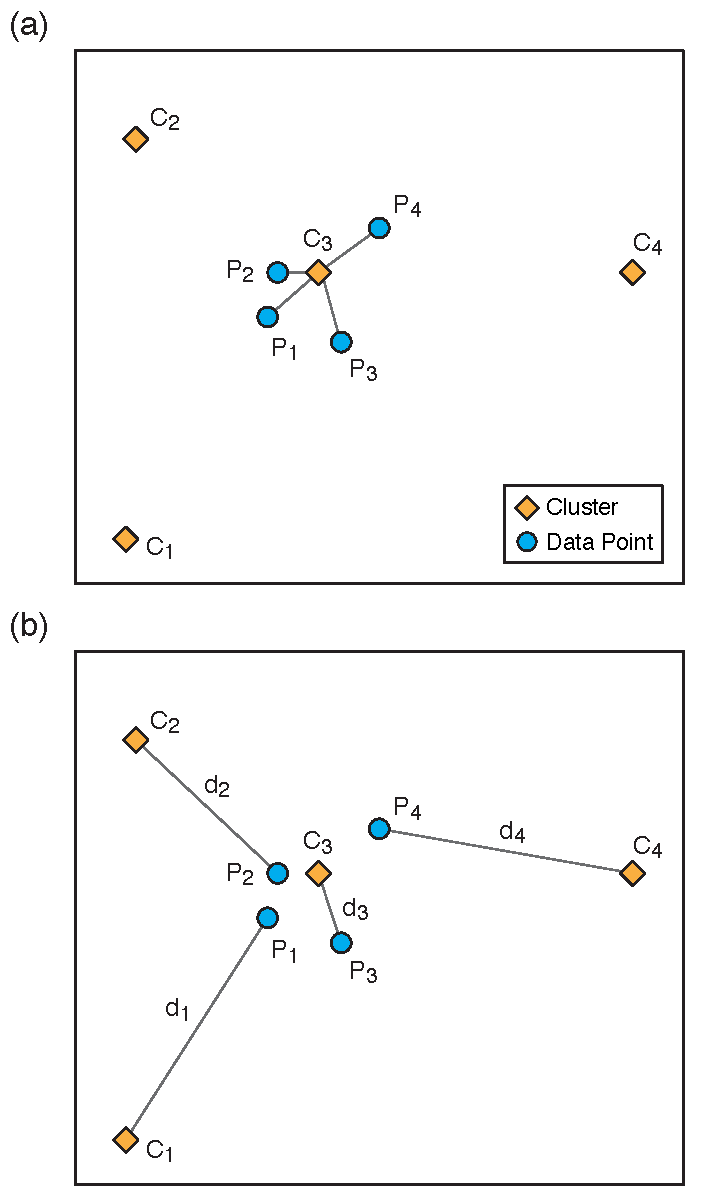
\includegraphics[width=\columnwidth]{figures/pdf/figure-04}
	\caption{Representation of the (a) ordinary, and (b) constrained \kmeans{} approaches for four data-points (P) and four cluster centers (C) in a 2D dataset space, where all the data-points are constrained to be cannot-link points. }
	\label{fig:k-means}
\end{figure}

In the multi-dimensional space defined by the 11 GOF metrics, the distance of each data-point to the cluster centers is done using the Euclidean distance:
% 
\begin{equation}
	d(x_i, x_j) = \sqrt{ \sum_{k=1}^{n} \left( x_{i,k} - x_{j,k} \right)^2 } 
	\, ,
\end{equation}
% 
where $n$ is the number of metrics, also called features, and $d$ is the distance between the data-points $x_i$ and $x_j$ in th $n$-$dimensional$ domain associated with the cluster $k$. Here, $x_i$ is the $i$-th feature value of the data-point $x$, and $x_j$ is the $j$-th feature value of the center of cluster. This is done for all $k$ clusters, thus the subindex $k$ on the right-hand-side terms.

It is, however, unpractical to expect the patterns defining the clusters to be observable using all the features at once. This is a common issue when clustering data in higher dimensions \citep[see, for instance,][]{Parsons_2004_ACM, Dy_2004_MLR}. A remedy to this problem is the use of sub-spaces, where clustering is limited to a number of dimensions or features. Here, we apply the constrained \kmeans{} method using sub-spaces with 2, 3, and 4 features. In total, we analyze 550 sub-spaces, 55 sub-spaces with 2 features, 165 with 3, and 330 with 4.

In the end, not all the sub-spaces will have clearly distinguishable clusters, or in other words, some will not satisfy the cannot-link constraints even after a large number of clustering iterations. Such sub-spaces are discarded, but in an ideal case, each station ends up being labeled 550 times. The final label applied to each station is the mode of the results. For example, if we name the labels $P$, $F$, $G$, and $E$ for poor, fair, good, and excellent, respectively, a station with final labels ${F F F P P G \dots E F F F F}$ will ultimately be labeled as $F$. Once all the data is properly labeled, we proceed with the decision tree analysis.


% ===========================================================================================
%


% Although we do not expect to see the pattern that resulted from clustering using 11 features in presentation of only two, however, different studies show that the higher dimension reduce the effect of similarity based on distance. \citet{Parsons_2004_ACM} presented an illustrative example to show the effect of dimension in reducing the importance of the distance. Effect of higher dimensions in clustering has been well studied and many different methods are proposed to reduce this effect in the final results. Among them we can name  feature selection before, during, and after clustering, hybrid methods that use combination of methods to select the best subset of feature. \citet{Dy_2004_MLR} addressed two issues involved in developing an automated feature subset selection algorithm for unlabeled data. They illustrated the irrelevant and redundant features and proposed methods for evaluating candidate features using two performance criteria.

% Subspace analysis is another technique to address the challenges with higher dimensional data in clustering process. Subspace clustering is an extension of traditional clustering which looks for different pattern using subset of features.  \citet{Parsons_2004_ACM} provided a list of algorithm for conducting subspace clustering and also some potential applications for them. The most common factor among these algorithm is the process to find a group of best subspaces through optimization process. An n-dimensional dataset has $2^n$ subspaces where it could be very costly and time consuming to evaluate all of them.

% In this study we are interested in using those features who, in general, represent the simulation accuracy in 4 different categories. As a first step we use the constrained \kmeans{} clustering approach for all features, however, because of mentioned reasons the results are not easy to discuss or even evaluate. Although we have four groups of data, the question is which one should be considered as poor, fair, good, or excellent groups. Therefore, we apply a modified method of subspace clustering approach to cluster the stations. As we discussed earlier and presented in figures the constrained \kmeans{} method effectively put the stations in a cluster with considering the fact that our constrain stations should not be in the same cluster. High number of iteration leads the clustering process to follow the clustering concept that we are looking for which is clustering stations as poor, fair, good, and excellent. In our case number of possible subspace is $2^{11}$ where each features have two options wether belong to subspace or not. However, because of preserving the distance based criteria effects we limited the number of features in the subspace to be 2,3, and 4 features. Therefor we have 330,165, and 55 unique subspaces for 4D,3D, and 2D, respectively. We conduct a constrained \kmeans{} clustering analysis for each of these subspaces and repeat the algorithm. In some cases, it is not possible to distinguish all four cannot-link stations in different clusters. In this study we ignore these cases. We only use those combination of features that gives 4 unique clusters for the constraint points (hypothetical stations), therefore, we know for sure that all data within same cluster let's say with metric value 3, should be considered as poor. We also control the clusters to be consistent (we reformat numbers to assign cluster 1 to all group of stations that our first constraint belongs to them and so on). Finally, using 550 unique subspace clustering results, we assign the most frequent class to the station.





% and computes . These distances are then used as a criteria to determine the cluster to which cluster each data-point belongs. 

% ...


% \citet{Macqueen_1967_Proc} describes this method as a process for partitioning a $n$-dimensional population into $k$ sets on the basis of a sample. Its algorithm produces partitions that are reasonably efficient in the sense of within-class variance. It starts with a user defined number of clusters ($k$) and assigns a random mean value to each cluster (or randomly choose $k$ data-points and assigns them as cluster centers). After this, the algorithm computes the distances of all other data-points to the center of the cluster and uses the distance as a criteria to clustering the data points. Because the data resides in a multi-dimensional space (here defined by each metric), there are different ways of computing the distance of each data-point to the cluster's center. We use the Euclidean distance:
% % 
% \begin{equation}
% 	d(x_i, x_j) = \sqrt{ \sum_{k=1}^{n} \left( x_{i,k} - x_{j,k} \right)^2 } 
% 	\, ,
% \end{equation}
% % 
% where $n$ is the number of features and $d$ is the distance of $x_i$ and $x_j$ in $n$-$dimensional$ domain. 




% ===========================================================================================
%
% NEW TEXT PROVIDED BY NAEEM ON JAN 22
% Once the distance is computed, the algorithms labels the data based on the proximity of each point to each cluster, and computes the arithmetic mean value of the data for each cluster, and assigne that value as the updated location of each cluster's center. The algorithm repeats the steps unless the amount of updates among the cluster centers is less than a predefined tolerance value. The major problem with \kmeans{} algorithm is that it is sensitive to the selection of the initial partition and may converge to a local minimum of the criterion function value if the initial partition is not properly chosen. Another problem accompanying the use of \kmeans{} algorithm is the choice of the number of desired output clusters. \citep{Jain_1999_ACMCS}. Clustering is a subjective process. The same set of data items often needs to be partitioned differently for different application. In our application the number of clusters according to the literature is 4 (i.e., poor, fair, good, and excellent.) However, our initial attempts represents that the results are highly sensitive to the initial clusters' center. Therefore, we need to incorporate the experts knowlege in the process. 


% \citet{Wagstaff_2001_Proc}  demonstrated a modification of \kmeans{} clustering algorithm which uses the background information of the domain or dataset. The algorithm adds two types of constraints to the clustering including:
% 	% 
% 	\begin{itemize}
% 	\item{Must-link: constraints specify that two instances have to be in the same cluster.}
% 	\item{Cannot-link: constraints specify that two instance must not be placed in the same cluster.}
% 	\end{itemize} 
% 	% 
% The algorithm is described in detail in \citet{Wagstaff_2001_Proc}, however, in simple words, in the ordinary \kmeans{} process before assigning data to the closes cluster, it controls the must-link and cannot-link conditions. Therefore, in this case, the closest cluster's center is not necessarily the final cluster of the data.


% In a hypothetical assumption, if we have a pair of data and synthetic with GOF score of 3 for all metrics we could consider the overall simulation GOF as poor. This is also correct for 5,7, and 9 that we can assigne them fair, good, and excellent class, respectively. Therefore, we add 4 hypothetical stations into the dataset with GOF score of 3,5,7,and 9 for all metrics and we put them in cannot-link constraint. This assumption that originated from the experts knowledge, provides enough information to the algorithm to converge to the same final clusters and cluster centers after a reasonable amount of iteration. 

% Fig.~\ref{fig:con_kmeans} presents the difference between ordinary and constrained k-means clustering approach using 4 points and 4 cluster centers. Fig.~\ref{fig:con_kmeans}.a presents the \kmeans{} without constrained. According to the definition and the explanation in this section, the closest cluster center for each points will get the points. 	Fig.~\ref{fig:con_kmeans}.b represents the constrained \kmeans{} approach, where, the closest cluster center is not necessarily the final cluster. The data points can not be in the same cluster, in result,  we assign them to different clusters in this case to satisfy the Cannot-link criteria. The best configuration happens when we minimize the distance between cluster centers and points.

% ===========================================================================================
% 
% OLD STUFF DONE BY RICARDO FOR THE INTRO OF THIS SECTION
% 
% In machine learning, decision trees are classified as a supervised learning method, and the first step towards designing them requires that the data be labeled according to their attributes. The inherent attribute of our data are the GOF value themselves, but because of the multiplicity of metrics and the lack of clarity about how these relate to each other, we need to add labels to the data that are in accordance with the outcome attributes, i.e., in terms of the predefined validation quality levels. We label the data in our dataset by means of a clustering process. 

% There exist different methods for clustering data \citep[see Chapters 10 and 11 in][]{Han_2011_Book}, among which the \kmeans{} and constrained \kmeans{} clustering methods are the most widely used \citep{Jain_1999_ACMCS}. We note about these methods that the \kmeans{} approach is sensitive to the initial values chosen to be at the center of the clusters---especially in the case of data that are not clearly distinguishable---, whereas the constrained \kmeans{} method uses background knowledge to overcome this limitation. Because of its use of background information, the modified \kmeans{} method is considered as a semi-supervised process.





% ===========================================================================================
%
% SECOND ATTEMPT THAT WAS RECALLED BY NAEEM

% Once the distance is computed, the algorithms labels the data based on the proximity of each point to each cluster, computes the mean value of the data for each cluster, and updates the location of each cluster's center. \textcolor{red}{(How do we compute ``mean value'' and how do we recompute the ``center''? All what follows after this in the original text is too descriptive, and not specific enough. We need to go to the point and this is going in long description circles.)} 

% {\color{gray}
% 	The algorithm repeats the steps unless the amount of updates among the cluster centers is less than a tolerance value.  \kmeans{} clustering has been applied in different applications, however, there is no clustering technique that is universally applicable in uncovering the variety of structures present in multidimensional datasets. Therefore, clustering is a subjective process. The same set of data items often needs to be partitioned differently for different application. In result, it is essential for the user of a clustering algorithm to not only have a thorough understanding of the particular technique being utilized, but also to know the details of the data gathering process and to have some domain expertise; the more information the user has about the data at hand, the more likely the algorithm would be able to succeed in assessing its true class structure. Domain concept can play several roles in the clustering process, and a variety of choices are available to the practitioner \citep{Jain_1999_ACMCS}. 

% 	The major problem with \kmeans{} algorithm is that it is sensitive to the selection of the initial partition and may converge to a local minimum of the criterion function value if the initial partition is not properly chosen. Another problem accompanying the use of \kmeans{} algorithm is the choice of the number of desired output clusters. Several variant of the \kmeans{} algorithm have been reported in the literature. Some of them attempt to select a good initial partition so that the algorithm is more likely to find the global minimum value, another variation is to permit splitting and merging of the resulting clusters \citep{Jain_1999_ACMCS}. 

% 	In our application the number of clusters is not a problem and there is a consensus among researchers in the number of clusters (i.e., poor, fair, good, excellent), however, our initial attempts represent that the results are highly sensitive to the initial clusters' center. 

% 	Every clustering algorithm uses some type of knowledge either implicitly or explicitly. In this study the background knowledge is a series of hypothetical stations. We assume that there are four stations with score of 3, 5, 7, and 9 for all of their metrics. Based on the score limits in section.~\ref{validation_metrics} we know these stations belong to poor, fair, good, and excellent classes, respectively. These background knowledge could help the clustering processing to be in right direction regarding the fact that increasing dimension of data could increase noise in clustering and cause difficulty to better partitioning. \citet{Wagstaff_2001_Proc}  demonstrated a modification of \kmeans{} clustering algorithm which uses the background information of the domain or dataset. The algorithm adds two types of constraints to the clustering including:
% 	% 
% 	\begin{itemize}
% 	\item{Must-link: constraints specify that two instances have to be in the same cluster.}
% 	\item{Cannot-link: constraints specify that two instance must not be placed in the same cluster.}
% 	\end{itemize} 
% 	% 
% 	The algorithm is described in detail in \citet{Wagstaff_2001_Proc}, however, in simple words, in the ordinary \kmeans{} process before assigning data to the closes cluster, it controls the must-link and cannot-link conditions. Therefore, in this case, the closest cluster's center is not necessarily the final cluster of the data. Fig.~\ref{fig:con_kmeans} presents the difference between ordinary and constrained k-means clustering approach using 4 points and 4 cluster centers. Fig.~\ref{fig:con_kmeans}.a presents the \kmeans{} without constrained. According to the definition and the explanation in this section, the closest cluster center for each points will get the points.
	
% 	Fig.~\ref{fig:con_kmeans}.b represents the constrained \kmeans{} approach, where, the closest cluster center is not necessarily the final cluster. The data points can not be in the same cluster, in result,  we assign them to different clusters in this case to satisfy the Cannot-link criteria. The best configuration happens when we minimize the distance between cluster centers and points. Using this method at each step the algorithm redistribute the 4 hypothetical stations to satisfy the cannot-link constraint. The visual inspection of the figures also confirms the accuracy of the method. Doing this, in the next iteration this data manipulation leads the cluster center in a direction to have the hypothetical station in the cluster and loose those data that is in far other side direction of the hypothetical station. Therefore, the cluster tend to have all data that similar to the hypothetical station. \\
% 	The end product of the clustering process is groups of data. Analysis of these groups, individually, gives the idea about the clusters in terms of within class variation. In these analysis we mainly study the behavior of different features in each cluster and isolate only the most descriptive features to be used in the supervised classifier that assumes a given number of classes in the data set. In the next section we provide a basics of decision tree algorithm. 

% }

% In other words, the points cannot be in the same cluster. In the constrained \kmeans{} approach we redistribute the points such that the $\sum{d}$ becomes minimum.

% ===========================================================================================
%
% OLD NAEEM VERSION
% 
% Clustering is an unsupervised approach for grouping of data based on measure of similarity and it is considered as an exploratory activity as a part of data mining process \citep{Fayyad_1996_IEEE}. In each valid cluster, patterns are more similar in each other than they are to pattern belonging to a different cluster. Many clustering algorithms are developed for different application, however, study the difference of them is beyond the scope of this paper. In general, at the top level,  \citet{Jain_1999} distinguished the clustering approach into Hierarchical and Partitional approaches. Aside from differences in application and technical details in implementation, hierarchical methods produce nested series of partitions, while partitional methods produce only one. In this study we are interested in using partitional, distance based clustering algorithm, which is also known as \kmeans{} algorithm.  \citet{Macqueen_1967_Proc}  described a process for partitioning an $n$-$dimensional$ population into $k$ sets on the basis of a sample. The process appears to give partitions which are reasonably efficient in the sense of within-class variance. For numerical values, \kmeans{} algorithm starts with a user defined number of clusters (k) and assign a random mean value for each cluster (or randomly choose k data and assign them as cluster centers.) Then it computes the distance of data and cluster centers. A variety of distance measures are in use in different studies, however, we use the Euclidean distance through 

% \begin{equation}
% d(x_i,x_j)=\sqrt{\Sigma_{k=1}^{n}(x_{i,k} - x_{j,k})^2},
% \end{equation}

% where $n$ is the number of features and $d$ is the distance of $x_i$ and $x_j$ in $n$-$dimensional$ domain. After computing the distance of the points from each clusters' mean (center), the algorithm continues with labeling the data after the closest cluster. At the next iteration, it computes the mean value of data for each cluster and updates the clusters' centers. The algorithm repeats the steps unless the amount of updates among the cluster centers is less than a tolerance value.  \kmeans{} clustering has been applied in different applications, however, there is no clustering technique that is universally applicable in uncovering the variety of structures present in multidimensional datasets. Therefore, clustering is a subjective process. The same set of data items often needs to be partitioned differently for different application. In result, it is essential for the user of a clustering algorithm to not only have a thorough understanding of the particular technique being utilized, but also to know the details of the data gathering process and to have some domain expertise; the more information the user has about the data at hand, the more likely the algorithm would be able to succeed in assessing its true class structure. Domain concept can play several roles in the clustering process, and a variety of choices are available to the practitioner \citep{Jain_1999}. 

% The major problem with \kmeans{} algorithm is that it is sensitive to the selection of the initial partition and may converge to a local minimum of the criterion function value if the initial partition is not properly chosen. Another problem accompanying the use of \kmeans{} algorithm is the choice of the number of desired output clusters. Several variant of the \kmeans{} algorithm have been reported in the literature. Some of them attempt to select a good initial partition so that the algorithm is more likely to find the global minimum value, another variation is to permit splitting and merging of the resulting clusters \citep{Jain_1999}. 

% In our application the number of clusters is not a problem and there is a consensus among researchers in the number of clusters (i.e., poor, fair, good, excellent), however, our initial attempts represent that the results are highly sensitive to the initial clusters' center. 

% Every clustering algorithm uses some type of knowledge either implicitly or explicitly. In this study the background knowledge is a series of hypothetical stations. We assume that there are four stations with score of 3, 5, 7, and 9 for all of their metrics. Based on the score limits in section.~\ref{validation_metrics} we know these stations belong to poor, fair, good, and excellent classes, respectively. These background knowledge could help the clustering processing to be in right direction regarding the fact that increasing dimension of data could increase noise in clustering and cause difficulty to better partitioning. \citet{Wagstaff_2001_Proc}  demonstrated a modification of \kmeans{} clustering algorithm which uses the background information of the domain or dataset. The algorithm adds two types of constraints to the clustering including:\\
% \begin{itemize}
% \item{Must-link: constraints specify that two instances have to be in the same cluster.}
% \item{Cannot-link: constraints specify that two instance must not be placed in the same cluster.}
% \end{itemize} 
% The algorithm is described in detail in \citet{Wagstaff_2001_Proc}, however, in simple words, in the ordinary \kmeans{} process before assigning data to the closes cluster, it controls the must-link and cannot-link conditions. Therefore, in this case, the closest cluster's center is not necessarily the final cluster of the data. Fig.~\ref{fig:con_kmeans} presents the difference between ordinary and constrained k-means clustering approach using 4 points and 4 cluster centers. Fig.~\ref{fig:con_kmeans}.a presents the \kmeans{} without constrained. According to the definition and the explanation in this section, the closest cluster center for each points will get the points.
% Fig.~\ref{fig:con_kmeans}.b represents the constrained \kmeans{} approach, where, the closest cluster center is not necessarily the final cluster. The data points can not be in the same cluster, in result,  we assign them to different clusters in this case to satisfy the Cannot-link criteria. The best configuration happens when we minimize the distance between cluster centers and points. Using this method at each step the algorithm redistribute the 4 hypothetical stations to satisfy the cannot-link constraint. The visual inspection of the figures also confirms the accuracy of the method. Doing this, in the next iteration this data manipulation leads the cluster center in a direction to have the hypothetical station in the cluster and loose those data that is in far other side direction of the hypothetical station. Therefore, the cluster tend to have all data that similar to the hypothetical station. \\
% The end product of the clustering process is groups of data. Analysis of these groups, individually, gives the idea about the clusters in terms of within class variation. In these analysis we mainly study the behavior of different features in each cluster and isolate only the most descriptive features to be used in the supervised classifier that assumes a given number of classes in the data set. In the next section we provide a basics of decision tree algorithm. 


% \begin{figure}
%     \centering
%     \includegraphics
%       %  [width=\columnwidth]
%         [width=200px]
%         {figures/pdf/Figure_4.pdf}
%     \caption{ Representation of ordinary (a) and constrained (b) \kmeans{} approach. There are four data points (p) and four cluster centers (c) as a sample of $2$-$Dimensional$ dataset. All points are defined as cannot-link constraints. In other words, the points cannot be in the same cluster. In the constrained \kmeans{} approach we redistribute the points such that the $\sum{d}$ becomes minimum.}
%     \label{fig:con_kmeans}
% \end{figure}

